% Editable explanatory figure. Schematic resources, not an experimental fixture.
\documentclass[border=4pt]{standalone}
\usepackage[T1]{fontenc}
\usepackage{lmodern}
\usepackage{tikz}
\usetikzlibrary{arrows.meta,positioning,calc}
\definecolor{ink}{HTML}{26343D}
\definecolor{accent}{HTML}{1F676D}
\definecolor{light}{HTML}{EEF5F5}
\begin{document}
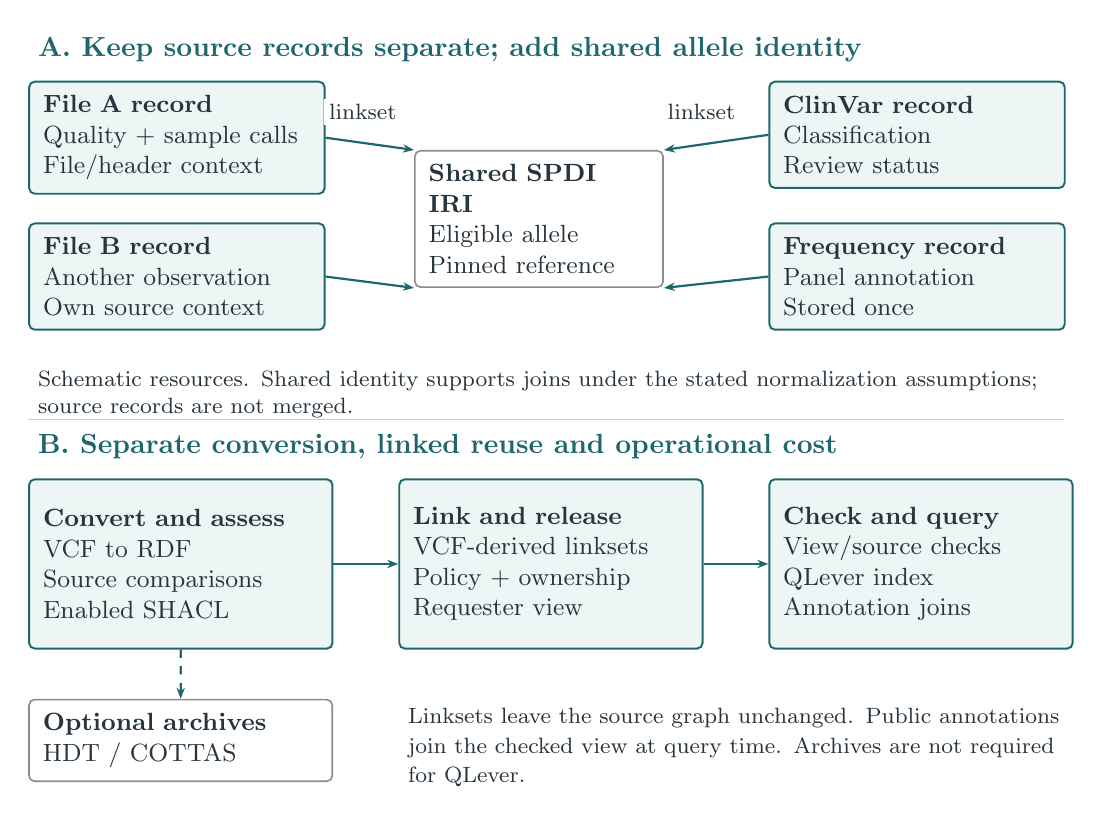
\begin{tikzpicture}[
 x=1cm,y=1cm,font=\fontsize{9}{11}\selectfont,text=ink,
 box/.style={draw=accent,fill=light,rounded corners=2pt,line width=.7pt,align=left,inner sep=5pt},
 plain/.style={draw=black!45,fill=white,rounded corners=2pt,line width=.6pt,align=left,inner sep=5pt},
 flow/.style={-{Stealth[length=4pt]},draw=accent,line width=.8pt},
 lab/.style={font=\fontsize{8}{9}\selectfont,fill=white,inner sep=2pt,align=center},
 head/.style={font=\fontsize{10}{12}\selectfont\bfseries,anchor=west,text=accent}
]

\node[head] at (0,0) {A. Keep source records separate; add shared allele identity};
\node[box,text width=3.4cm,minimum height=1.35cm,anchor=north west] (a) at (0,-.4) {\textbf{File A record}\\Quality + sample calls\\File/header context};
\node[box,text width=3.4cm,minimum height=1.35cm,anchor=north west] (b) at (0,-2.2) {\textbf{File B record}\\Another observation\\Own source context};
\node[plain,text width=2.8cm,minimum height=1.4cm,anchor=north west] (id) at (4.9,-1.28) {\textbf{Shared SPDI IRI}\\Eligible allele\\Pinned reference};
\node[box,text width=3.4cm,minimum height=1.35cm,anchor=north west] (cv) at (9.4,-.4) {\textbf{ClinVar record}\\Classification\\Review status};
\node[box,text width=3.4cm,minimum height=1.35cm,anchor=north west] (af) at (9.4,-2.2) {\textbf{Frequency record}\\Panel annotation\\Stored once};
\draw[flow] (a.east) -- (id.north west);
\draw[flow] (b.east) -- (id.south west);
\draw[flow] (cv.west) -- (id.north east);
\draw[flow] (af.west) -- (id.south east);
\node[lab] at (4.25,-.8) {linkset};
\node[lab] at (8.55,-.8) {linkset};
\node[anchor=north west,text width=12.8cm,font=\fontsize{8}{10}\selectfont] at (0,-3.96) {Schematic resources. Shared identity supports joins under the stated normalization assumptions; source records are not merged.};
\draw[black!20] (0,-4.7) -- (13.15,-4.7);
\node[head] at (0,-5.05) {B. Separate conversion, linked reuse and operational cost};
\node[box,text width=3.5cm,minimum height=2.15cm,anchor=north west] (con) at (0,-5.45) {\textbf{Convert and assess}\\VCF to RDF\\Source comparisons\\Enabled SHACL};
\node[box,text width=3.5cm,minimum height=2.15cm,anchor=north west] (pol) at (4.7,-5.45) {\textbf{Link and release}\\VCF-derived linksets\\Policy + ownership\\Requester view};
\node[box,text width=3.5cm,minimum height=2.15cm,anchor=north west] (que) at (9.4,-5.45) {\textbf{Check and query}\\View/source checks\\QLever index\\Annotation joins};
\draw[flow] (con.east) -- (pol.west);
\draw[flow] (pol.east) -- (que.west);
\node[plain,text width=3.5cm,minimum height=1cm,anchor=north west] (arc) at (0,-8.25) {\textbf{Optional archives}\\HDT / COTTAS};
\draw[flow,dashed] (con.south) -- (arc.north);
\node[anchor=north west,text width=8.45cm,align=left,font=\fontsize{8.5}{10.5}\selectfont] at (4.7,-8.25) {Linksets leave the source graph unchanged. Public annotations join the checked view at query time. Archives are not required for QLever.};
\end{tikzpicture}
\end{document}
